\documentclass[12pt, oldlfont, amsfonts]{report}
\usepackage{cmap}					% поиск в PDF
\usepackage[T2A]{fontenc}			% кодировка
\usepackage[utf8]{inputenc}			% кодировка исходного текста
\usepackage[english,russian]{babel}	% локализация и переносы
\usepackage{amssymb}
\usepackage{graphicx}
\usepackage{cellspace}
\setlength\cellspacetoplimit{14pt}
\usepackage{etoolbox}
\usepackage[a4paper, includefoot,top=20mm, bottom=20mm, right=10mm, left=30mm]{geometry}
%\usepackage[T1]{fontenc}
%\usepackage{calligra}
%\usepackage{frcursive}

\usepackage[english,russian]{babel}
\usepackage{graphicx}
\graphicspath{ {./figs/} }
\usepackage[export]{adjustbox}
\usepackage{siunitx}
\usepackage{titlesec} %отступы

\renewcommand {\baselinestretch}{1.5}
\renewcommand{\theequation}{\arabic{section}.\arabic{equation}}
%\renewcommand{\thetable}{\thesection.\arabic{table}}.
%\renewcommand{\thetable}{\arabic{chapter}.\arabic{table}}
\renewcommand\normalsize{\fontsize{14}{14pt}\selectfont}



\makeatletter
% запрещаем переносы в названиях секций
\renewcommand{\section}{\@startsection{section}{1}{0pt}%
                                {-3.5ex plus -1ex minus -.2ex}%
                                {2.3ex plus .2ex}%
{\centering\hyphenpenalty=10000\normalfont\Large\bfseries}}

% меняем заголовок для команды \chapter и запрещаем переносы слов
\usepackage {titlesec}
\titleformat{\chapter}{\thispagestyle{plain}\centering\hyphenpenalty=10000\normalfont\large\bfseries}{
\thechapter. }{0pt}{\Huge}


%изменить название главы "Литература" на "Список использованных источников":

\addto\captionsrussian{\renewcommand\bibname{Список использованных источников}}


%чтобы метки списка литературы были не стандартно в квадратных скобках:
\makeatletter
\renewcommand\@biblabel[1]{#1.}
\makeatother

% Рисунок вместо Рис. и тире вместо двоеточия
\makeatletter
\renewcommand{\fnum@figure}{Рисунок \thefigure \ -- }
%\patchcmd{\@makecaption}{#1: #2}{#1}{}{}
\patchcmd{\@makecaption}{#1: #2}
  {#1\sbox8{#2}\ifdim\wd8=\z@\else #2\fi}
  {}{\ddt}

\makeatother
\titlespacing*{\chapter}{0pt}{-40pt}{20pt}
\setlength\parindent{1.25cm}


\pagestyle{empty}
\begin{document}
    \newpage
    \begin{center}
    \linespread{1}
		Министерство науки и высшего образования  Российской Федерации\\
федеральное государственное бюджетное образовательное учреждение\\
высшего образования\\
«Иркутский государственный университет»\\
(ФГБОУ ВО «ИГУ»)\\
Факультет бизнес-коммуникаций и информатики 
    \end{center}
\vspace{1cm}    
\hspace{8cm} 
\begin{minipage}{0.5\textwidth}
\linespread{1}
  \begin{flushleft}
	\small{
    Кафедра естественнонаучных дисцсплин \\%\vspace{-2cm}
Допускается к защите \\
и.о. зав. кафедрой, к.ф.-м.н., доцент \\
\_\_\_\_\_\_\_А.Г. Балахчи\\
		«\_\_\_»\_\_\_\_\_\_\_\_\_ 202\_ г \\		}
		%\vspace{2еm}
		
		
		%\vspace{4.0em}
		\end{flushleft}
\end{minipage}


    \vspace{2cm}
    \begin{center}
   {\bf КУРСОВАЯ РАБОТА\\
    по направлению  \\
		09.03.03 Прикладная информатика\\
		%\vspace{1em}
		профиль\\
		«Разработка программного обеспечения»\\}
    \end{center}
		
		%\vspace{2.5em}
    \begin{center}
  		Разработка бота для изучения "Прикладной математики и теории вероятности" в телеграмм \\
    \end{center}
		
		\vspace{0.5em}
		
   \hspace{-5em} 



\begin{minipage}[t]{0.5\textwidth}
  \begin{flushleft}
  
		\end{flushleft}
\end{minipage}\hspace{1em} 
\begin{minipage}[t]{0.5\textwidth}
  \begin{flushleft}
  \linespread{1}
	\small{
    Студент 3 курса
	очной формы обучения \\
  группа 14323\\
	\_\_\_\_\_\_Ковязин Степан Андреевич\\
	\vspace{2em}
		
	Руководитель: преподаватель\\
		\_\_\_\_\_\_Сокольникова Александра Константиновна\\
\vspace{2em}
 Работа защищена:\\
	«\_\_\_»\_\_\_\_\_\_\_\_\_ 2023 г \\
 с оценкой \_\_\_\_\_\_\\
Протокол № \_\_\_}
		%\vspace{2em}
		
		
		%\vspace{4.0em}
		\end{flushleft}
\end{minipage}

    \vspace{\fill}
\vspace{1em}
    \begin{center}
   {\bf Иркутск 2023  }
    \end{center}
\newpage

\pagestyle{plain}%headings

\newpage
\setcounter{page}{2} 
\newpage

\tableofcontents % это оглавление, которое генерируется автоматически


\setcounter{chapter}{0}
\setcounter{subsection}{0}
\setcounter{equation}{0}
\setcounter{section}{0}

\chapter*{\large{{\centering ВВЕДЕНИЕ}}}
\addcontentsline{toc}{chapter}{ВВЕДЕНИЕ}

Актуальность темы курсовой работы обусловлена тем, что в современном мире каждый может, с помощью различных конструкторов, собрать своего собственного бота. Человек, который умеет программировать и пользоваться базами данных, способен написать более умного бота, который, например, мог бы отслеживать действия каждого и быстрее взаимодействовать с пользователем. В телеграмме можно разработать бота, который будет устраивать различные викторины, опросы, но до сих пор тяжело встретить в свободном доступе бота, что предоставлял пользователю теоретическую информацию по какому-либо предмету, и затем проверить, как он усвоил выученный материал. 
	
Объектом исследования являются телеграмм боты, а предметом исследования процесс работы.

Целью курсовой работы является разработка телеграмм бота, который предоставляет пользователю: 
\begin{enumerate}
\item Выполнение теста по выученному материалу, набранные баллы по выбранному тесту сохраняются в базе данных до следующего повторного прохождения;
\item 	Сравнение результатов выполненного теста с другими пользователями, что также выполнили данный тест.
\end{enumerate}
	
Задачи курсовой работы:
\begin{enumerate}
\item Изучить на каком языке программирования и среде разработки можно написать телеграмм бота;
\item Изучить базы данных и определиться с выбором;
\item Придумать логику и структуру бота;
\item Начать разработку;
\item Тестировать рабочую часть бота, если всё в порядке, то переходим к другой части бота;
\item По окончанию разработки необходимо произвести тестовый запуск с пользователями для отлова возможных багов;
\item Если баги обнаружены, устраняем их;
\item Разработать веб-приложение для обслуживания базы данных бота.
\end{enumerate}

\setcounter{section}{0}
\setcounter{subsection}{0}
\setcounter{subsubsection}{0}
\setcounter{equation}{0}
\setcounter{section}{0}

\chapter{\large{ВЫБОР ИНСТРУМЕНТОВ ДЛЯ РЕШЕНИЯ ПОСТАВЛЕННОЙ ЗАДАЧИ}}
Бота возможно реализовать на любом современном языке – Java, Ruby, JavaScript и тд. Но был выбран python, у него есть необходимые библиотеки для разработки telegram бота, а так же на нём проще и быстрее его реализовать. Помимо python не менее популярны так же php и Java Script, Но разработка на них сложнее и дольше. Так же веб-приложение будет писаться на python. Поэтому бот и веб-приложение будут в одном проекте.
	
Средой разработки для Python был выбран PyCharm, он обладает рядом преимуществ, таких как:
\begin{enumerate}
\item PyCharm предназначен именно для Python, значит как только его установишь, создаешь файл или проект и можешь сразу начать писать код, не переживая ни о чём;
\item Простая организация проектов – легко создать новый проект и открыть уже существующий, буквально в пару кликов можно открыть проект и уже начать писать;
\item Прекрасный автокомплит – срабатывает мгновенно, не нужно его вызывать;
\item Прекрасный интерфейс – данная среда имеет английский текст, но даже не зная его, можно интуитивно понять, что, как и где делается;
\item Очень много горячих клавиш;
\item Встроенный терминал – нужен для удобной установки библиотек.
\end{enumerate}	

Если даже не учитывать эти плюсы, я бы всё равно выбрал PyCharm для Python, поскольку пишу в нём давно и привык к нему.

Для разработки использовалась библиотека telebot, она легко осваивается новичком, и есть все основные функции. Выбор пал на неё потому, что в ней имеются все необходимые именно для меня функции.

В качестве базы данных была выбрана MySQL, потому что, по моему мнению, это идеальная база практически для чего угодно, и для telegram бота так же подходит идеально.

Для создания веб-приложения также будет использоваться среда разработки PyCharm с использованием библиотеки flask.

\chapter{\large{РАЗРАБОТКА БОТА}}
\section{Создание бота, создание проекта и установка библиотеки}
Для начала необходимо создать бота в telegram с помощью другого бота в telegram, для этого необходимо: 

\begin{enumerate}
\item В telegram ищем бота по имени  @BotFather и нажимаем start;
\item Пишем команду /newbot и вводим имя бота;
\item После придумываем username;
\end{enumerate}	

После всего проделанного получаем токен созданного бота. токен в telegram боте - это средство идентификации в виде зашифрованной последовательности символов. Поэтому его нельзя передавать другим.

Теперь создаём проект в среде разработки PyCharm:
\begin{enumerate}
\item В открываем PyCharm и нажимаем new Project;
\item В открывшемся окне вводим название нашего нового проекта;
\item Нажимаем create и открывается проект с python файлом main.
\end{enumerate}

Проект создан, в нём мы будем разрабатывать нашего бота и веб приложение. Нам нужно сразу задать структуру проекта. Первым делом создадём новую директорию с названием bot и в ней python файл \_\_init\_\_. Теперь папка bot является пакетом.

Пакет в Python – это каталог, включающий в себя другие каталоги и модули, но при этом дополнительно содержащий файл \_\_init\_\_.

В директории бот создадём директории: buttons, courses, database, functions, handlers.

Со структурой пакета bot разобрались. Вне пакета создаём файл .env, в ней мы храним переменные, которые нельзя видеть другим пользователям, если мы захотим выложить наш проект на gitHub. В созданном файле моздаём переменную token и записываем в неё наш токен. 

Теперь необходимо инициализировать бота. Открываем терминал и вводим pip install pytelegrambotapi. Таким образом мы скачиваем библиотеку telebot. Так же необходимо скачать {\bf python-dotenv}. С помощью библиотеки dotenv мы можем использовать переменные из файла { .env}.

В пакете bot в файле { init} импортируем библиотеки telebot,os и и dotenv. Создаём переменную bot и записываем в неё { telebot.TeleBot(os.getenv('token'))}. Теперь пишем декоратор { @bot.message\_handler(commands=['start'])} и функцию, вызываемую с помощью данного декоратора. С помощью данного декоратора мы будем обрабатывать команду start от пользователя. При обработке команды бот должен отправить 'Привет' пользователю. Мы написали приветствующего бота, теперь его необходимо запустить, запускать мы будем из python файла main вне пакета бот. Для этого из пакета bot импортируем переменную bot и затем пишем { bot.polling(none\_stop=True)}. Запускаем программу и проверяем. Дмонстрацию работы можно увидеть на рисунке 2.1.


\begin{figure}[h!]
\center{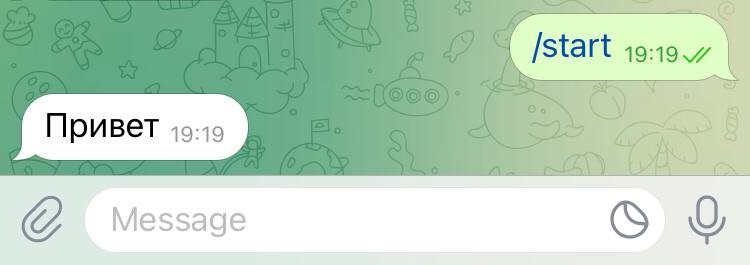
\includegraphics[width=0.8\linewidth]{1.jpeg}}
\caption{Демонстрация работы приветствующего бота}
\label{fig:1.jpeg}
\end{figure}

 
\section{Подключение базы данных к боту}
Теперь, когда мы инициализировали бота, ему нужно определять, подключался ли прежде пользователь к боту или он сделал это в первый раз. Создаём базу данных и в ней таблицу с названием { users} и полями { id} и { user}.

\begin{enumerate}
\item { id} - Уникальный идентификатор пользователя;
\item { user} - id пользователя в telegram.
\end{enumerate}	
Переходим в файл { .env} и создаём переменные { host},{ dbname}, { user} и { password}. В переменных сохраняем данные базы данных.

Создаём в папке database python файл MySQLConnect. Скачиваем библиотеку { pymysql}. В файл импортируем библиотеки pymysql,os и dotenv. Создаём функцию { create\_connection} и с помощью { pymysql.connect} создаём и возвращем из функции соединение с БД. 

В папке database создаём python файл { personalDataOfUsers}, импортируем функцию { create\_connection}. Создаём две функции, одна для { поиска} пользователя, а другая для { добавления} пользователя. В этих функциях мы пишем { SQL запросы} ДБ и проверяем, подключался ли пользователь к боту прежде, если нет, то нужно добавить его { id} в таблицу.

Создаём в папке handlers python файл { handlerStart}, в нём мы будем обрабатывать команду { start} от пользователя. Сначала мы проверяем наличие пользователя в базе, если он есть, тогда для того, чтобы не захламлялся чат, удаляем последние 2 сообщения и затем пишем { С возвращением, мы рады снова вас видеть!!!}, в ином случае { Добро пожаловать на наш канал, я бот, обучающий математике.}  и добавляем пользователя в БД.

Мы успешно подключили БД к боту, пеперь можно проверять. Демонстрацию работы можно увидеть на рисунке 2.2


\begin{figure}[h!]
\center{
\includegraphics[width=0.8\linewidth]{2.jpeg}}
\caption{Демонстрация работы бота c подключённой БД}

\end{figure}


 
\section{Разработка функции отправки текста курса для обучения}

Теперь необходимо расширить функционал бота. Начнём с разработки вывода текста для обучения. В папке buttons создаём python файл buttonsMenu, из библиотеки telebot импортируем класс types, создаём {bf функцию для генерации кнопок меню}. В нашем случае { меню} - это { домашняя страница}, когда пользователь использует команду { start}, то переходит именно на эту страницу. Говоря страница, имеется ввиду не буквально страница, а ориентация относительно разделов бота. Пока из кнопок меню есть только { курсы}, но количество кнопок пополнится по мере разработки бота. Теперь создадём в папке { handlers} python файл { handlerCourses} и в нём обработчик кнопки { курсы}, при клике на кнопку должен вывестись список кнопок с названиями курсов.

Названия курсов должны откуда-то браться, в нашем случае из БД, поэтому создаём в БД таблицу с названием { courses} и полями { id}, { name}, { callback}, { file\_path}, { status}.

\begin{enumerate}
\item { id} - Уникальный идентификатор курса;
\item { name} - наименование курса, именно это будет видеть пользователь при выборе курса;
\item { callback} - идентификатор курса для бота, именно с помощью него бот будет понимать, какой курс выбрал пользователь;
\item { status} - статус курса, по нему определяется, отображается ли курс у пользователя или нет, сейчас он не нужен, но будет использован при создании веб приложения.
\end{enumerate}	

В папке { database} создаём python файл {coursesRequest}, импортируем функцию { create\_connection} и создаём функцию для получения { списка курсов}. Мы можем получать список курсов, и теперь необходимо преобразовать их в кнопки.

В папке { buttons} создаём python файл { buttonsCourses}, импортируем python файл { coursesRequest} и { types} из telebot и создаём функцию для генерации кнопок.

Мы создали все необходимые функции для вывода кнопок с курсами, теперь проанализируем работу обработчика кнопки { курсы}, сначала происходит обращение к функции генерации кнопок списка из файла { buttonsCourse}, из этой функции происходит обращение к функции для получения списка курсов из БД в файле { coursesRequest}, полученный список возвращается в функцию генерации кнопок, и по этому списку в цикле генерируются кнопки с курсами, и по окончанию цикла так же к списку добавляется кнопка с возвратом в { главное меню}. Сгенерированные кнопки возвращаются в обработчик и результат отправляется пользователю.

Мы ещё не написали обработчик для возврата в главное меню, в файле { handlerCourses} добавляем обработчик для возврата в главное меню.

Теперь мы имеем список кнопок с курсами, нам необходимо выводить эти курсы. Для того, чтобы пользователь мог спокойно их просматривать, ему нельзя выдавать весь текст сразу, а в виде страниц, или дозировано, допустим, по 1000 символов. И где то нужно хранить прогресс прочтения курса. В БД создаём таблицу с названием { users activity in courses} и полями { id},{ user\_id}, { course\_id}, { is\_passing}, { send\_symbols}, { max\_size\_course}.
\begin{enumerate}
\item { id} - уникальный идентификатор активности пользователя;
\item { user id} - id пользователя, который ссылается на первичный ключ таблицы { users}, именно по нему определяется к какому пользователю относится активность;
\item { course id} - id курса, который ссылается на первичный ключ таблицы { courses}, именно по нему определяется какой курс изучает или изучал пользователь;
\item { is passing} - по ней мы определяем, что именно этот курс в данный момент изучает пользователь, имеет значение 0 или 1;
\item { send symbols} - по ней определяем, сколько текста в символах мы отправили пользователю, не может быть больше { max size course};
\item { max size course} - количество символов в документе с курсом.
\end{enumerate}	
В файле { handlerCourses} необходимо написать обработчик нажатия на кнопку с выбранным курсом. Создаём переменную, в которой будем хранить активность пользователя. В файле { personalDataOfUsers} создаём две функции, первая будет искать пользователя в таблице с историей по просмотру курса, если пользователь смотрел курс прежде, то передаём в переменную активность пользователя, иначе в другой функции создаём новую активность по выбранному курсу. 

Создаём python файл { funcCourse} с импортом файлов { coursesRequest}, { personalDataOfUsers} и { buttonsCourse}.
Создаём функцию для получения текста курса исходя из данных пользователя и выбранного им курса.

Функция для получения текста работает следующим образом, у нас есть документ откуда мы берём текст, допустим, в тексте 10000 символов. По нажатию на кнопку с названием курса, мы передаём в функцию название курса, файл с этим курсом считывается, мы хотим вывести пользователю не весь текст, а только 1000, поэтому проверяем, сколько текста пользователь уже прочитал, если это новый пользователь, то он ничего не прочитал, значит количество выведенных символов равно 0 и так же это значит, что ему нужно вывести в диапозоне от 0 до 0+1000 символов, так же нужно вывести кнопки для перелистывания текста, мы проверяем,если текущее выведеное количество символов - 1000 меньше или равно 0, то выводим кнопки { главное меню} и { Следующая}, в ином случае выдаём кнопки { предыдущая}, { следующая} и { главное меню}.

Создадём python файл { buttonsCourser}, в нём создаём функцию для вывода кнопок для перемотки текста. Именно в этом файле генерируются кнопки для перелистывания текста.

Создаём в папке { handlers} python файл {handlerCourse}, в ней создаём функции для обработки нажатия кнопок  { предыдущая}, { следующая} и { главное меню}.

По такому же принципу работают и кнопки для перелистывания текста, после изменения диапозона они по такому же принципу проверяют, какие кнопки выводить.

Вот мы и создали все необходимые функции, проанализируем работу.

Обрататываем нажатие кнопки с курсом, ищем в БД данные о просмотре курса прежде пользователем, если он прежде открывал курс, то сохраняем в переменную полученную активность, иначе создаём новую активность по данному курсу и сохраняем её в переменную, затем полученные данные передаём в функцию для получения текста, в функции мы считываем .txt файл с курсом и делаем срез символов и возвращаем полученный текст, теперь обращаемся к функции для получения кнопок и возвращаем кнопки для перелистывания текста.
У нас имеются кнопки и текст, их отправляем пользователю.



У пользователя имеется возможность выбрать курс для изучения. При выборе пользователем курса, происходит обработка нажатия, из нажатой кнопки бот узнаёт, какой курс пользователь желает получить и проверяет в БД, смотрел ли пользователь данный курс прежде, если ответ положительный, то пользователю выводится текст с того же места, где он закончил, в ином случае текст выводится сначала. Пользователь может комфортно изучать курс, когда устанет, может закрыть и продолжить чтение позже с того же места. Так же текст подаётся частично с возможностью перелистывать его вперёд или назад.

\section{Разработка функции тесты}
Вот мы и добрались, по моему мнению, до самого сложного, выполнение тестов пользователем. Помимо кнопки курсы мы должны создать кнопку тесты, при переходе по этой кнопке будут показаны все доступные тесты для выполнения, мы выполняем тест только один раз и узнаём свои результаты, выполнить тест повторно можно будет только лишь если тест подвергнется изменениям.

Обновим кнопки, в python файле { buttonsMenu}, Добавляем кнопку { тесты}.

Теперь в БД необходимо создать таблицу { tests}. создаём таблицу { tests} с полями { id}, { name}, { callback}, { status}.

\begin{enumerate}
\item { id} - Уникальный идентификатор теста;
\item { name} - наименование теста, именно это будет видеть пользователь при выборе теста;
\item { callback} - идентификатор теста для бота, именно с помощью него бот будет понимать, какой тест выбрал пользователь;
\item { status} - статус теста, по нему определяется, отображается ли тест у пользователя или нет, сейчас он не нужен, но будет использован при создании веб приложения.
\end{enumerate}	


В папке database создаём python файл { testRequest}, создаём в нём функцию для получения списка тестов.

В папке buttons создаём python файл { buttonsTest} в нём мы генерируем кнопки с тестами.

В папке handlers создаём файл { handlerTests}, создаём в нём функцию обработчик для отлавливания нажатия кнопки { тесты}. 

Так же сразу создаём обработчик для кнопки возврата в меню из раздела { tests}.

Проанализируем работу кнопки. При нажатии кнопки { тесты} отлавливается нажатие кнопки, обработчик обращается к функции генерации кнопок, функция генерации кнопок обращается к функции для получения списка тестов и получает список тестов и БД, затем в цикле генерирует кнопки и передаёт в обработчик. Обработчик отправляет полученный результат пользователю.

Мы имеем список тестов, теперь необходимо решить, где будут храниться вопросы и варианты ответов для тестов. Для этого создадим две таблицы. В БД создаём таблицу { questions} с полями { id}, { test id} и { question}. в этой таблице мы храним { id} теста и { вопрос} к нему. 
\begin{enumerate}
\item { id} - уникальный идентификатор вопроса;
\item { test id} - id теста, который ссылается на первичный ключ таблицы { tests}, именно по нему определяется к какому тесту относится вопрос;
\item { question} - вопрос для теста.
\end{enumerate}	

В БД создаём таблицу { answers} с полями { id}, { question id}, { answer option} и { answer}.
\begin{enumerate}
\item { id} - уникальный идентификатор варианта ответа;
\item { question id} - id вопроса, который ссылается на первичный ключ таблицы { questins}, именно по нему определяется к какому вопросу относится вариант ответа;
\item { answer option} - вариант ответа для вопроса;
\item {answer} - определяет является ли вариант ответа верным, имеет значение 0 или 1.
\end{enumerate}	
Теперь у нас есть возможность хранить вопросы и варианты ответов для них, но ещё нам нужно где-то хранить прогресс пользователя, для этого создаём в БД ещё одну таблицу { users activity in test} с полями { id}, { user id}, { test id}, { num question}, { is passing}, { is passed}, { result} и { max result}.
\begin{enumerate}
\item { id} - уникальный идентификатор вопроса;
\item { user id} - id пользователя, который ссылается на первичный ключ таблицы { users}, именно по нему определяется к какому пользователю относится активность;
\item { test id} - id теста, который ссылается на первичный ключ таблицы { tests}, именно по нему определяется какой тест выполняет или выполнял пользователь;
\item { num question} - номер вопроса, на котором остановился пользователь;
\item { is passing} - по ней мы определяем, что именно этот тест в данный момент выполняет пользователь, имеет значение 0 или 1;
\item { is passed} - по ней определяем, закончил ли пользователь выполнение теста, под выполнением подразумевается полное окончание теста, имеет значение 0 или 1;
\item { result} - результат выполнения теста пользователем, не может быть больше максимального результата, при правильном ответе результат увеличивается;
\item { max result} - максимально возможный результат, определяется путём подсчёта количества вопросов в тесте. 
\end{enumerate}	
В данной таблице мы отслеживаем какой { тест} выполняет пользователь и его { прогресс}. 

В python файле { handlerTest} создаём обработчик для выбранного теста.

В python файле { personalDataOfUser} добавляем 2 функции, первая для поиска и получения активности пользователя по выбранному тесту, вторая для создания активности в случае её отсутствия в БД.

После получения активности пользователя, нам нужно вывести вопрос и варианты ответов. Для этого создаём python файл { funcTest} и создаём функцию для получения вопросов и вариантов ответов. Так же в данной функции мы проверяем, достигли ли мы конца теста. На самом деле данная функция скорее обращается к другим функциям для получения вопросов и вариантов ответов, но это лучше, чем из обработчика обращаться к разным функциям, гораздо лучше обратиться к одной функции, которая обратится к другим функциям и сведёт результат в виде словаря. 

Создаём в python файле { testsRequest} функцию для получения вопросов, функция работает следующим образом, мы передаём в неё индекс нужного вопроса и нужный тест, функция обращается к БД и получает список вопросов по выбранному тесту, мы возвращает из всего списка нужный вопрос по индексу. 

Создаём python файл { buttonsTest} и в ней функцию для генерации кнопок с вариантами ответов. Из функции для получения вопросов и вариантов ответов после получения вопроса мы этот вопрос передаём в нашу функцию генерации кнопок, данная функция передаёт данный вопрос в python файле { testsRequest} в функцию для получения вариантов ответа, и по вопросу мы получаем варианты ответов и возвращаем результат в функцию генерации кнопок, в цикле генерируются кнопки и так же по окончанию цикла добавляется кнопка возврата в меню, если вдрруг пользователь затрудняется ответить и решил перечитать курс.

Теперь при нажатии кнопки теста у нас будет выводиться вопрос и варианты ответа и сейчас нам нужно написать обработчик для выбора варианта ответа, то есть когда пользователь нажимает на вариант ответа, нам нужно проверить,является ли он правильным, если да, то дать ему один балл, если нет, то ничего, и вывести правильный и неправильные варианты ответов и добавить кнопку далее, чтобы пользователь мог включить следующий вопрос. 

В python файле { handlerTest} пишем обработчик выбранного варианта ответа, в обработчике мы в переменную записываем тест, который выполняется пользователем, для этого в python файле { testsRequest} пишем функцию, определяющую, какой тест выполняет пользователь по его { id} и возвращаем результат по id, дальше нам нужно получить снова получить активность пользователя из функции, передав в функцию полученный тест и { id} пользователя. Потом проверяется, какой вариант ответа выбрал пользователь, если правильный, то в данных пользователя к результату прибавляем 1 балл, иначе ничего не делаем. После проверки результата мы обращаемся к функции для получения выполняемого вопроса, передав в неё выполняемый тест и индекс вопроса, вопрос нам нужен для того, чтобы получить варианты ответов к нему. В python файле создаём функцию для получения правильного ответа, именно в эту функцию мы передаём полученный вопрос, эта функция обращается к функции для получения вариантов ответа из файла python { testRequest}, передавая вопрос, и по получению вариантов ответа формирует текст, в котором отмечечается,правильный ответ или нет. Полученный текст возвращается обратно в обработчик. Прежде чем его отправлять пользователю, нам так же нужна кнопка { следующий}, для этого в python файле { buttonsTest} создаём функцию для генерации кнопки, и полученный результат возвращаем в обработчик. Полученный текст и кнопку отправляем пользователю, затем в активности пользователя к номеру вопроса добавляем один, эту активность нужно сохранить, поэтому в python файле { personal data of users} создаём функцию для обновления активности пользователя на сервере.

При нажатии кнопки следующий, должен открыться следующий вопрос, для этой кнопки так же нужно написать обработчик,работает он следующим образом, обращается к функции для поиска выполняемого пользователем теста по { id} пользователя, затем функция возвращает полученный результат, дальше мы обращаемся к функции поиска и получения активности пользователя передавая в неё выполняемый тест и id пользователя, затем после получения активности обращаемся к функции для получения вопроса и вариантам ответа, так же в этой функции мы определяем, закончил ли пользователь тест или нет с помощью сравнения вопроса пользователя и количества вопроса в тесте, если пользователь прошёл тест, то отправляем ему текст с результатом и кнопку завершить,а в БД отмечаем что он прошёл тест и при попытке пройти снова будем выводить ему текст,что он уже прошёл тест и второй раз пройти нельзя, иначе отправляем вопрос и варианты ответа. Кнопка завершить возвращает пользователя в главное меню.

На этом моменте разработка функции выполнения тестов в боте завершена. 

Теперь нужно проанализировать то, как бот будет работать со стороны пользователя. Пользователь нажимает тесты, получает список тестов для выполнения, бот проверяет, выполнял ли пользователь прежде тест, если выполнял, то пользователя сообщат о том, что он уже выполнял тест, и больше не может его выполнить. В ином случае бот выводит вопрос с вариантами ответа, пользователь выбирает один из них, затем ему выводятся в виде текста правильные и неправильные варианты ответа и кнопка следующий, при нажатии бот проверяет, является ли выполненный вопрос последним, если да, то сообщаем пользователю результат и кнопку { завершить}, иначе выводим следующий вопрос с вариантами ответа.



\section{Разработка функции результаты}
Нам необходимо разработать функцию для возможности просмотра результатов уже выполненных тестов.

Обновим кнопки, в python файле { buttonsMenu}, Добавляем кнопку { результаты}.

Создаём python файл { handler result tests} и пишем обработчик кнопки { результаты}. В данном обработчике мы обращаемся к функции для формирования текста о результатах пользователя в тестах, для этого создаём python файл { funcResult} и в ней необходимую функцию. Данная функция обращается к БД для получения всех тестов, затем полученный список тестов проводит через цикл, просматривая в активности пользователя, выполнял ли он данный тест или нет. Если тест выполнялся, но не закончен, то пишем, что тест ещё не выполнен, если выполнен, то считаем в процентах сколько правильных ответов, если пользователь вообще не выполнял тест, то пишем что тест ещё не выполнялся, полученный текст отправляем пользователю и добавляем кнопку для возврата в меню.



\section{Подведение итогов главы}

Мы разработали бота, с помощью которого пользователь может обучаться математике. Были разработаны функции: изучение курса по той или иной теме, выполнение тестов и просмотр результатов по выполненным тестам.

\chapter{\large{{РАЗРАБОТКА ВЕБ ПРИЛОЖЕНИЯ ДЛЯ ОБСЛУЖИВАНИЯ БОТА}}}
\section{Создание структуры веб приложения, установка библиотек и создание экземпляра приложения}
Веб приложение для бота нам нужно для его обслуживания, через него мы будем добавлять и изменять тесты и курсы, а так же доступ у к веб приложению будет только у создателя бота. Веб приложение должно иметь чёткую структуру для облегчения разработки и обслуживания. Создаём в проекте пакет { web\_app}.Скачиваем библиотеку flask. В python файл { init} импортируем библиотеку flask и создаём экземпляр приложения { app=Flask(\_\_name\_\_)}. В пакете создаём папки: { database}, { static}, { templates} и views. Это стандартная структура проекта на flask кроме папки database.
\begin{enumerate}
\item { static} - в данной папке хранятся { js}, { css} и { img} файлы;
\item { templates} - в данной папке хранятся { html} страницы и шаблон;
\item { views} - в данной папке хранятся python файлы c функциями представления;
\item { database} - в данной папке хранятся python файлы с функциями для обращения к БД.
\end{enumerate}	



\section{Создание страницы для авторизации}
Поскольку через это приложение обслуживается бот, то нельзя чтобы в него мог зайти любой пользователь, поэтому необходимо создать страницу для авторизации пользователей. Страницы для регистрации не будет, поскольку веб приложение пишется исключительно под данного бота.

Для начала создадим в папке { templates} html файл {auth}, в нём мы будем верстать нашу страницу. В папке { static} создадим папку {css}, в ней мы будем хранить стилевые файлы для страниц, а в этой папке папку {auth} и в ней css файл { auth\_style}. именно этот стилевой файл будет использоваться для страницы авторизации. Так же необходимо в папке {static} создать папку { img}, в ней будут содержаться все изображения, используемые на сайте, а данный момент мы добавляем в неё логотип нашего сайта. Логотип можно увидеть на рисунке 3.1.
\begin{figure}[h!]
\center{
\includegraphics[width=0.8\linewidth]{3.png}}
\caption{логотип сайта}
\end{figure}

Теперь необходимо создать функцию представления чтобы к странице можно было обратиться по {url} адресу. Создаём в папке { views} python файл { auth} и импортируем наш экземпляр приложения. В файле создаём функцию представления { @app.route('/login', methods=['get', 'post'])} и в ней возвращаем страницу пользователя.

Теперь к странице можно обратиться по { url}. Демонстрацию страницы авторизации можно увидеть на рисунке 3.2.
\begin{figure}[h!]
\center{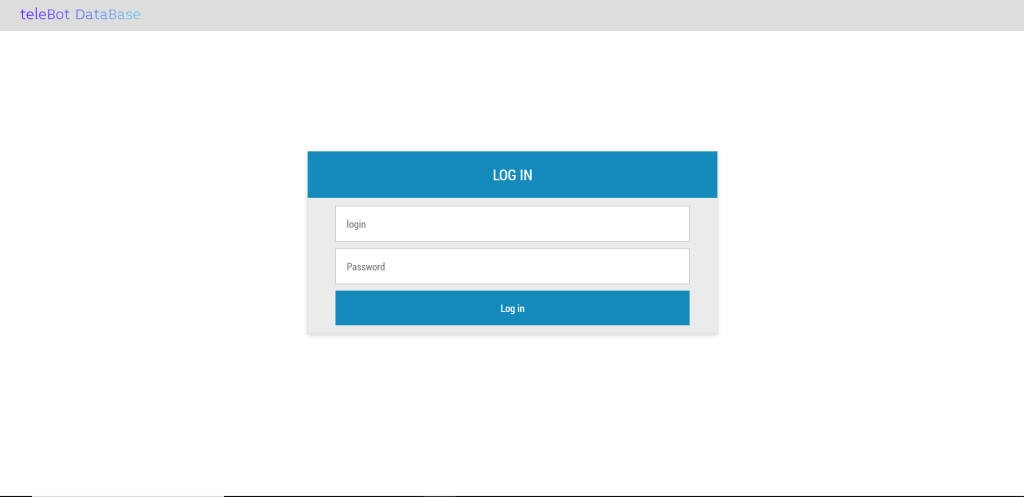
\includegraphics[width=0.6\linewidth]{4.jpeg}}
\caption{страница авторизации}
\end{figure}

Сейчас мы можем просмотреть страницу авторизации, но в дальнейшем к ней смогут перейти лишь не авторизованные пользователи или точнее будут насильно перемеены для авторизации, поскольку все страницы будут доступны лишь авторизированным пользователям. Для того,чтобы пользователь мог авторизоваться, нужно чтобы его данные были в БД, создаём таблицу { app account} с полями { id}, { username}, { login}, { password}.

\begin{enumerate}
\item { id} - Уникальный идентификатор пользователя для авторизации;
\item { username} - имя пользователя на сайте;
\item { login} - логин для авторизации;
\item { password} - пароль для авторизации.
\end{enumerate}

И в данной таблице создаём пользователя, указав { username}, { login} и { password}.

Во flask есть расширение { flask-login}, оно позволяет интегрировать аутентификацию в приложение. Скачиваем библиотеку { flask-login} и импортируем в файл { init}. Для использования flask-login из неё импортируем класс { LoginManager} и создаём новый экземпляр { LoginManager}. Поскольку мы работаем с БД, то нам нужно скачать библиотеку { flask sqlalchemy}, он является расширением flask и используется для соединения с БД и у нас будет использоваться только для авторизации. Создаём новый экземпляр { sqlalchemy} в переменной { db}. Для проверки пользователей нужно создать класс { User}, именно с помощью него мы проверяем пользователя и авторизовываем. Создаём python файл { models} и импортируем в него из файла { init} переменные { LoginManager} и { db}, из { flask-login} { UserMixin}. В этом файле мы создаём класс { User} и передаём импортированные { db} и { UserMixin}. В классе обращаемся к таблице { app account} - { \_\_tablename\_\_ = 'app account'}, и 4 переменных: { id}, { username}, { login} и { password}.

Из написаного не совсем понятно, что мы сделали, поэтому необходимо разобрать созданный класс. Созданный нами класс является моделью таблицы, к которой мы обращаемся, обычно название класса является названием таблицы, но если мы не хотим чтобы название класса совпадал с названием таблицы, то переменной { \_\_tablename\_\_} нужно задать явное название таблицы. { \_\_tablename\_\_} - это специальная переменная класса, используемая для определения имени таблицы базы данных. Созданные  4 переменные являются экземпляром класса { db.column}, с помощью { column} мы явно указываем, какой столбец таблицы мы хотим получить, например поле { id} имеет тип { int} и является первичный ключом, выглядит так { db.Column(db.Integer, primary\_key=True)}. Так же в классе есть { UserMixin}, он по умолчанию реализует методы: is\_authenticated, is\_active, is\_anonymous, и сработает только тогда, когда сработает функция загрузчика пользователя. В данный класс передаются { логин} и { пароль} отправленные пользователем, но рассмотрим это чуть позднее. В данный файл мы импортировали переменную { login manager}, сейчас её и применим. Создаём под классом декоратор { @login manager.user loader}. Благодаря ему при успешной авторизации {flask-login} обращается к классу { app account} и теперь срабатывает {UserMixin} он делает пользователя авторизованным и { flask login} запоминает авторизованного пользователя.

В { init} файле была создана переменная { db}, но не было подключения к конкретной БД, подключаемся к БД { app.config['SQLALCHEMY DATABASE URI'] = 'mysql+pymysql://user:@host/database'}. Теперь мы имеем подключение к нашей БД и можно дальше разрабатывать страницу регистрации, а именно нам нужно обработать ответ сервера при отправке формы с логином и паролем. 

Обрабатывать будем { POST} запрос с данной страницы по адресу { /login}. В функции представления { /login} пишем { POST} обработчик, сначала проверяем, является ли запрос { POST}, если является, то проверяем, указал ли пользователь логин и пароль, если указал, то отправляет в класс { User}, в качестве ответа получаем id пользователя или none, если не найден пользователь, когда мы получили пользователя, в login\_user передаём его { id} и авторизовываем пользователя, и он автоматически переходит на ту страницу, которую хотел.



\section{Создание шаблона страницы}
До этого мы создавали html страницу авторизации, которая являлась уникальной сама по себе, последующие две страницы управление курсами и управление тестами очень похожи друг на друга, поэтому чтобы не писать их с нуля, мы напишем шаблон страницы. В шаблоне будет { header} и { навигационное меню по страницам}.

Создадим в папке { templates} html файл { base} именно он будет являться шаблоном наших будущих страниц. 

  папке static создаём папку { js}, чуть позднее заполним её, а так же в папке { css} создаём css файл { style}, именно он будет являться стилевым файлом нашего шаблона.

Начнём разработку нашей страницы. В теге { body} создаём контейнер { div} с классом { window}. В данном контейнере в первую очередь создаём боковое навигационное меню. В верху меню добавляем логотип сайта, а под ним перечисляем страницы для перехода. Теперь в контейнере с классом { window} создаём шапку нашей страницы. В правом краю шапки создаём надпись пользователь, после отображаем имя авторизованного пользователя и кнопку выйти.

Написали нашу страницу шаблон, теперь на неё нужно перейти, мы будем отображать имя авторизованного пользователя, поэтому и было начать первым делом разработка страницы авторизации. В python файле { views} создаём функцию представления { @app.route("/base")} и добавляем под ней декоратор { @login\_required}, данный декоратор не позволяет перейти на страницу неавторизованным пользователям. И в данной функции представления возвращаем нашу html страницу. Шаблон страницы можно увидеть на рисунке 3.3.

\begin{figure}[h!]
\center{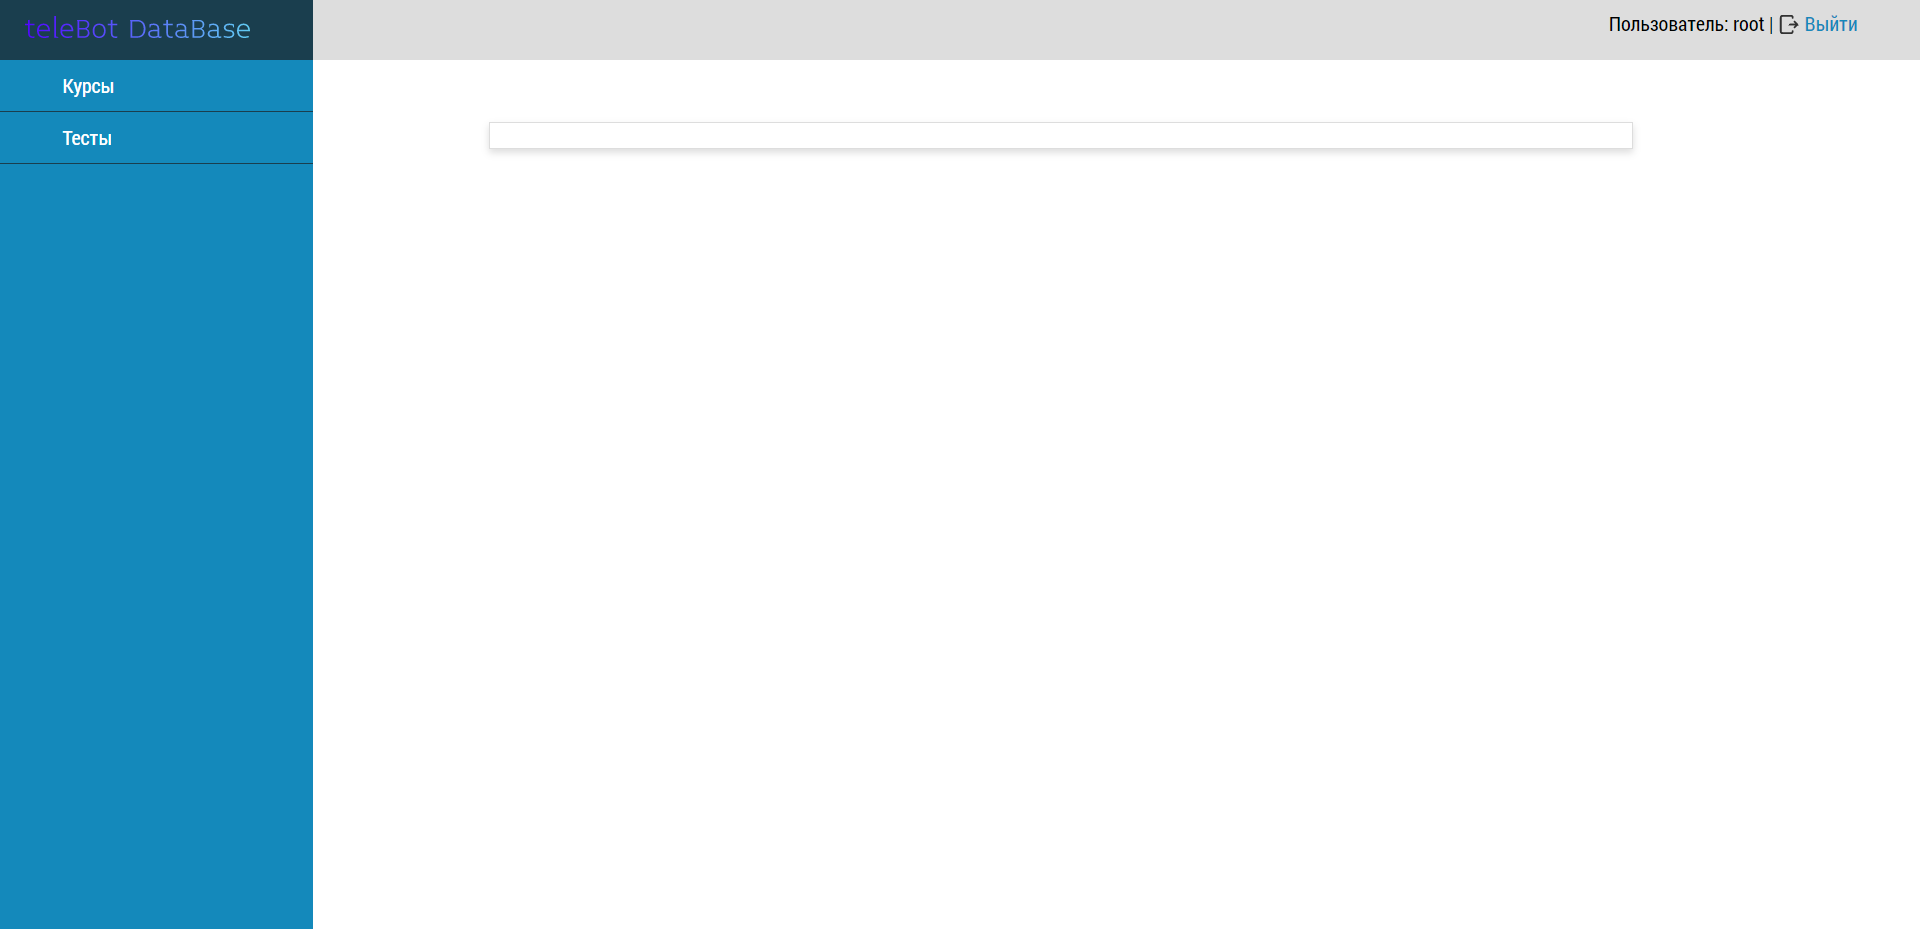
\includegraphics[width=0.8\linewidth]{7.png}}
\caption{шаблон страниц}
\end{figure}

Получился неплохой шаблон, но теперь нам необходимо адаптировать страницу для устройств низкого разрешения, поскольку если экран будет меньше 1000px, то страница будет ощущаться переполненной. Для данной страницы при маленьком разрешении будет достаточно сделать боковое навигационное меню выдвижным чтобы освободить пространство будущему контенту на странице.

Для начала создадим в папке { js} файл { viewport}, в этом файле мы отслеживаем размер страницы, и в случае, если страница по ширине меньше 1080px, то скрываем боковое меню и добавляем кнопку для его вывода, а если больше 1080, то возвращаем обратно боковое меню без возможности скрытия. Для управления этим процессом создаём в той же папке js файл { menu-style} здесь мы создаём функцию для вывода и скрытия бокового меню, и функцию для ослеживания клика когда меню выдвинуто, если клик был вне меню, то скрываем его.  

Мы ещё не закончили разработку шаблона страницы, поскольку в ней нет { плейсхолдеров}. { плейсхолдеры} - это ячейки с динамическим содержанием, индивидуальной для каждой страницы, используемой шаблон и заключены в секции {{... }}, одна секция содержит одну переменную, значение переменной передаётся в процессе генерации страницы в функции представления. Так же есть условные операторы внутри блоков \{ \{ \% ... \%\}\}, в такие блоки можно передавать множество html кода или просто текста отображаемого на странице. Именно эти блоки нужно создать в наш шаблон, в них мы будем выводить содержимое новых страниц. Для начала в теге { head} пропишем блок {scripts}, в неё мы будем передавать элементы тега { head} из страниц, используемых шаблон. Так же в теге div с классом { container} добавим блоки { containerHeaderContent} и { content}, в первом блоке мы будем выводить то, какая это страница, а на второй выводить содержимое.



\section{Создание страницы тесты}
В папке { templates} создаём html файл {tests}, все html файлы в папке { templates} являются шаблонами, как бы это странно ни звучало, но разница в том, что есть родительский шаблон, а так же дочерний, html файл {base} является родительским, в созданном файле {tests} первой строкой пишем \{\{\% extends "base.html" \%\}\}, этот тег является ключевым,он сообщает механизмам шаблонов, что этот шаблон расширяет другой шаблон, то есть содержимое { base} передаём в { tests}. Теперь при вызове html файла {tests} мы получаем такую же страницу как и { base}. Теперь заполняем блоки { containerHeaderContent} и { content}, созданные в шаблоне. В блоке { containerHeaderContent} пишем раздел сайта, в нашем случае раздел { тесты}, и добавляем кнопку { добавить тест}. С блоком { content} всё сложнее, мы хотим получить все тесты из базы данных в виде списка на странице, значит будем использовать условные операторы, но нам необходимо получить тесты из БД, значит в папке { database} создаём python файл { MySQLConnect} и в нём создаём функцию подключения к БД аналогичную функции в боте, так же в папке создаём python файл { tests\_DB}, в него импортируем нашу функцию подключения к БД и создаём функцию для получения тестов из базы данных. В python файл { views} импортируем файл { tests\_BD}, создаём функцию представления для html файла tests и при генерации страницы передаём ей полученный из БД список тестов. Теперь в html файле {tests} можно дальше работать с блоком { content}, в нём проходимся в цикле по списку тестов, нам нужно сгенерировать для каждого вопроса в списке контейнер, в котором в левой части мы указываем кликабельное имя теста, чтобы при нажатии на него перейти на страницу с вопросами, в правой чекбокс со статусом, имеющим значение 0 или 1, как и говорилось в главе с разработкой бота, статус нужен будет при разработке приложения,так же кроме чекбокса создаём кнопки редактирования и удаления теста. Полученные контейнеры отображаем на странице в виде списка. С созданием разметки закончили, теперь нужно создать и применить стили, в папке { css} создаём папку { tests}, так мы явно разделяем стили для каждой страницы и в этой папке создаём два css файла { style box content} и { style header content}, с одной стороны кажется странным, что мы не применяем стили в одном файле, но с другой мы чётко можем понять, в каком блоке какие стили применяются и где они используются, что облегчит изменение стиля каких либо элементов в блоках. В блоке { scripts} применяем эти стилевые файлы. Проверим, что мы сделали, к странице можно перейти по адресу { /tests}, для проверки уже создано пару тестов. Посмотреть как это выглядит на сайте можно на рисунке 3.4.
\begin{figure}[h!]
\center{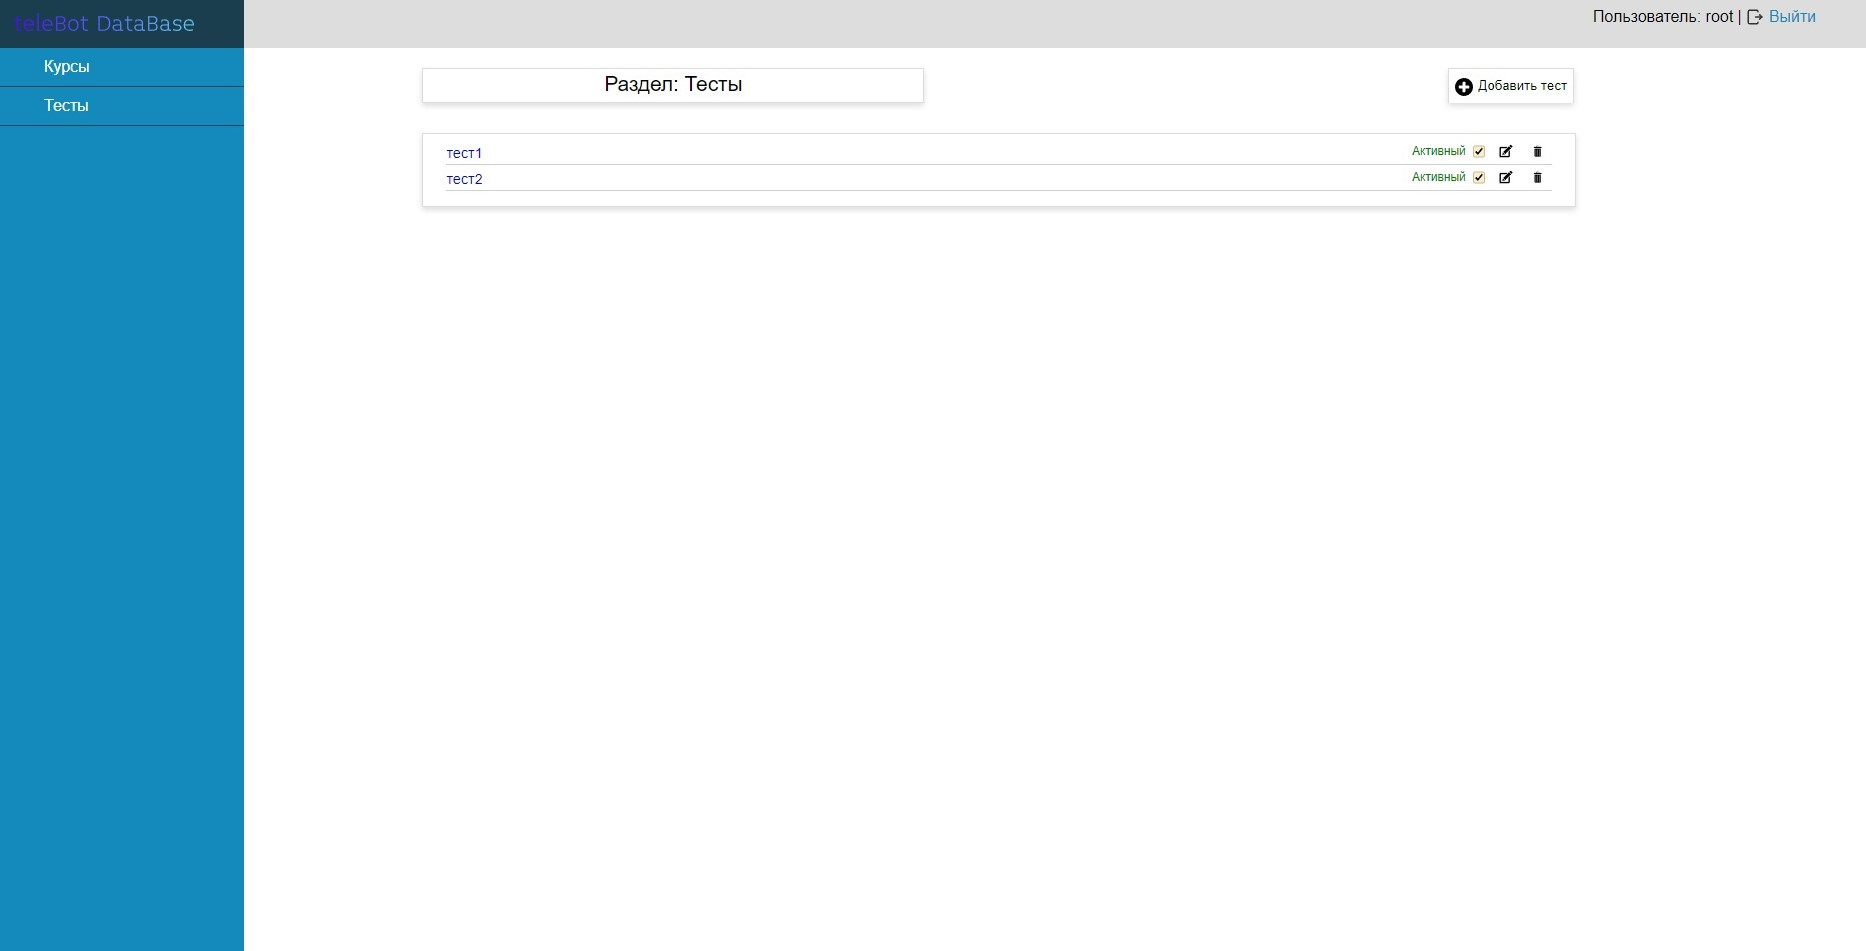
\includegraphics[width=0.8\linewidth]{8.jpg}}
\caption{страница тесты}
\end{figure}

Убедились, что всё работает как надо, но на странице есть кнопки и они ничего не делают, исправим это. Для начала реализуем работу кнопки редактировать, в файле js создаём папку { tests} и в ней js файл { edit name}, в файле создаём функцию { edit name}. Функция работает следующим образом, мы нажимаем на кнопку нужного теста, тег span с именем теста заменяется на поле input в фокусе, содержащий старое название теста, после проверяем, находится ли поле в фокусе, если нет, то мы удаляем пробелы из значения в поле input, затем проверяем условия: 
\begin{enumerate}
\item { не пустое значение} - значение в поле input не должно быть пустым;
\item { уникальное название} - новое зазвание теста не должно совпадать с другими тестами;
\item { не совпадать со старым названием} - новое название не должно быть как предыдущее название теста.
\end{enumerate}

должны пройти все эти условия, иначе возвращаем старое название, для применения нового названия так же можно убрать поле из фокуса или нажать на клавишу { enter}, а для отката нажать клавишу { esc}. Для проверки всех этих условий мы не использовали БД по той причине, что это требует времени, да, это было бы надёжнее, но скорость важнее. Так же для применения нового названия нужно обновить название так же в БД, и хочется чтобы обращение к серверу происходило без обновления страницы, для этого используем функцию  { \$.ajax} из библиотеки { JQuery}. Создаём в { js/tests} js файл { scripts ajax}, в нём мы храним функции с { \$.ajax} для обращения к серверу, эти функции находятся в другом файле для удобства обслуживания. Ajax имеет параметры, которые необходимо указать:

\begin{enumerate}
\item { url} - куда мы отправляем данные;
\item { method} - метод { get/post};
\item { contentType} - тип содержимого, передаваемого на сервер;
\item { data} - данные, которые будут отправляться на сервер. 
\end{enumerate}

В файле { scripts ajax} создаём функцию { edit name ajax} и пишем ajax функцию, к какому же url мы будем отправляться, а отправляться будем в { /\_edit\_name}, а значит нужно создать функцию представления для { url}, создаём в папке { views} python файл { tests\_func}, в нём нужную нам функцию представления и обрабатываем запрос { post} , а именно, принимаем переданные переменные и отправляем в python файле { tests\_DB} в функцию для запроса в БД для изменения названия теста. Функция представления должна что-то возвращать, неважно что, главное не пустой ответ и не значения { int}, в нашем случае передаём { '0'}, если функция ajax выполнилась успешно, то обрабатывает функцию для параметра { success}. Не совсем понятно, что мы сделали, поэтому необходимо проанализировать работу, анализируем с того момента, как новое название теста прошло все условия. Мы обращаемся к функции с {ajax} и передаём { id} и { новое имя теста}, в ajax эти данные передаются на сервер там эти переменные отправляются в функцию для запросов в БД, и отпраляется запрос на изменение имени теста в тесте с конкретным { id}, затем функция представления должна вернуть что-либо, поскольку мы не получаем из БД, а меняем, то получить оттуда нечего, значит возвращаем ноль с типом { String}, затем в ajax вызывается функция {success}, она вызывается, если ajax отработал провильно и запрос был выполнен, в нём мы меняем на странице название теста на новое. В разработке следующих функций будем опускать процесс создания функции представления, запросов к БД, поскольку процесс такой же, будем лишь описывать, как работает функция для кнопки. 

Теперь реализовываем функцию для кнопки удаления, создаём js файл {delete} и в ней функцию, при удалении проверяем, что статус теста равен 0, то есть отключен и другим пользователям это не доставит проблем, после по id удаляем тест в БД, а на странице просто стираем этот контейнер. 

Теперь функция смены статуса, при изменении чекбокса, текст, который показываем статус так же меняем, сначала проверяем, что мы хотим сделать, активным или нет, если делаем активным тест, то проверяем наличие вопросов, если вопросов нет, то не позволяем тесту стать активным, если всё хорошо и вопросы есть, то меняем статус и текст, который показывает статус и сбрасываем данные пользователей по данному тесту, поскольку мы могли поменять вопросы, а так же блокируем переход на страницу с вопросами, если тест активен, чтобы нельзя было менять вопросы, пока кто-то делает тест. Если делаем тест неактивным, то просто в БД меняем статус теста на ноль.

Функция для кнопки добавления тестов, как же ж без неё, создаём js файл { add test} и в ней функцию, при нажатии на кнопку создаём пустой контейнер в конце списка и добавляем в него поле input, условия те же, что и при редактировании названия, кроме несовпадения со старым именем, поскольку его нет, уникальность имени, не пустое значение. После этого нажимаем {enter} и новый тест создаётся в БД, возвращаем его id и дополняем созданный контейнер, присваиваем ему id, добавляем чекбокс и кнопки редактировать и удалить.

Создали все функции, но мы ещё их не применили, то есть они есть, но не привязаны к своим кнопкам, создаём js файл {action buttons}, и к каждой кнопке присваиваем функцию, к кнопкам в списке не надо привязывать функции к каждой, поскольку путь к кнопкам совпадает.

Теперь все созданные скрипты привязываем к нашей html странице, вносим их в блок { scripts}, для файла { action buttons} дополнительно добавить атрибут defer, это значит, что скрипт применится только после полного создания документа, это нужно затем, что скрипты загружаются в порядке прогрузки документа, то есть если скрипт находится на первой строчке, то сначала загрузится он а потом и страница, но если элемент, что используется в скрипте, ещё не существует на странице, то будет ошибка.

Теперь всё работает, но есть ещё одна проблема, уведомления, вроде мелочь, но сложно понять, что идёт не так пользователю, допустим он не заметил, что пытается удалить активный тест и знает почему не получается, но если бы всплыло уведомление, он бы его прочитал и всё понял. В интернете уже написано столько скриптов для уведомлений, что я считаю, не смысла изобретать то, что уже существует. Есть библиотека js { JQuery.toast}, она поставляется вместе с css файлом, скачиваем его перекидываем в папку js, а его css в папку css и применяем их в странице шаблоне, поскольку уведомления нужны будут на других страницах, применение у данной библиотеки простое, есть функция с параметрами, переносим в неё такие парамерты как, тема уведомления, например успех или провал, текст уведомления и цвет фона, цветом мы показываем, какое уведомление, плохое или хорошее.



\section{Создание страницы тест}
В данном параграфе мы будем разрабатывать страницу, на которой будем редактировать сам тест, то есть создавать вопросы и варианты ответа к ним.

В папке { templates} создаём html файл {test}, используем страницу шаблон. В python файле views создаём функцию представления для нашей страницы, мы передаём в неё { id} нашего теста, и тем самым открываем вопросы именно нужного теста. Путь url у неё { /tests/id}, где id это id нашего теста. Так же делаем в функции представления проверку на то, активен ли наш тест, если да, то перекидываем пользователя на страницу со всеми тестами. Иначе открываем ему страницу с вопросами. В html файле {test} заполняем блок { containerHeaderContent} в нём мы создаём поле, где показываем, какой тест обновляем, а ниже пишем, что это раздел { вопросы} и делаем кнопку { добавить вопрос}, в блоке { content} так же у нас будет список, аналогичный списку на странице tests, но без чекбокса со статусом и при клике не переводящий на другую страницу, добавление вариантов ответа реализовывать будем на этой же странице. Для получения вопросов нам нужно обратиться к БД, но поскольку это уже другая страница, лучше будет создать новый файл, в папке database создаём python файл { test\_DB} и создаём там функцию для получения вопросов, результат передаём в функцию представления, где и преобразуется уже на странице в виде списка. Заполнили блоки, теперь необходимо подключить стилевые файлы, в папке { css} создаём папку { css-test} и в ней два файла: { style box content} и { style header content}.  Так же у нас будет модальное окно для работы с вопросом, а именно: создание, редактирование, удаление и смена правильного ответа. Создавать его будем через js скрипт, у нас есть вопросы, которые уже существуют, а есть те, которые будут создаваться, и подход к ним отличается, поэтому id у окна будет отличаться в зависимости от того, что мы делаем, но это чуть позднее, сейчас привяжем функцию создания вопроса к кнопке для создания вопросов. Создаём в папке js файл { scripts ajax} и папку {new question}, в созданной папке создаём js файл {create question} и в нём функцию { create question}. Работает функция следующим образом, создаётся контейнер с полем input, пользователь вводит название вопроса и нажимает { enter}, в функции проверяется введённый вопрос, он должен не быть пустым и являться уникальным для данного теста, после соблюдения этих условий мы обращаемся к функции для открытия модального окна, не сохраняем вопрос сразу по той причине, что пользователь может передумать создавать вопрос и вопрос то он уже создал, но не заполнил его, то есть нет вариантов ответа. Создаём в папке { new question} js файл { show modal window} и функцию для вывода окна, в переменной js пишем html код модального окна, у него должна быть шапка с названием вопроса, блок с вариантами ответов и внизу две кнопки для отмены и сохранения. Выводим модальное окно на странице, и в этой же функции чуть позднее создадим функции для кнопок сохранить и отмена.

Теперь у нас имеется модальное окно, пишем функцию для создания варианта ответа. Создаём js файл {create answer option}, данная функция так же выводит контейнер с input, мы вводим вариант ответа и он должен быть уникальным к данному вопросу и не пустым. При соответствии этим условиям убираем input и в span вносим имя варианта, на правой стороне контейнера распологаем radiobox для выбора правильного варианта ответа, кнопки редактировать и удалить, и в функции ниже привязываем функции для этих кнопок.

Теперь функция для редактирования варианта ответа, создаём js файл { edit answer option} и в нём функцию для редактирования варианта ответа так же проверяем на уникальность и не пустоту, и в случае соблюдения условий меняем текст варианта ответа. Для функции удаления варианта ответа создаём js файл { delete answer option} и пишем в нём функцию для удаления варианта ответа, в нашем случае просто удаляем контейнер, без каких либо проверок, поскольку этого не требуется. И остаётся функция для смены правильного варианта ответа, создаём js файл { changing true answer option} и в ней функцию для смены варианта ответа, работает это следующим образом, пользователь нажимает на { radiobox}, все подписи меняются на { не правильный ответ} и затем на выбранном меняем надпись на { правильный ответ}. Мы написали все функции для кнопок внутри контейнера с вариантом ответа у создаваемого вопроса. Теперь создадим функции для кнопок { отмена} и { сохранить}. Создаём js файл { cancel} и пишем в ней функцию для отмены, она закрывает модальное окно и удаляет последний контейнер с создаваемым вопросом в списке. Теперь создаём функцию сохранения, создаём js файл { save answer option and question} и в нём функцию сохранения. Работает функция следующим образом, мы проверяем варианты ответа, должны соблюдаться следующие условия: количество вариантов ответа минимум два и среди них выбран правильный ответ. После соблюдения этих условий добавляем вопрос в БД, получаем его { id}, варианты ответа заносим в массив и отправляет массив с { id} созданного вопроса в БД где в цикле построчно занесётся каждый вариант ответа в таблицу. После добавляем атрибут { id} в контейнер с вопросом и закрываем модальное окно.

С созданием новых вопросов и вариантов ответа разобрались, теперь напишем функции для кнопок удаления и редактирования вопросов. Создаём js файл { edit question} и функцию для редактирования вопроса, превращаем имя вопроса в поле input, вводим новое название,как и описывалось не один раз ранее при редактировании новое название должно быть уникальным, не быть пустой строкой и не являться таким же, как предыдущее название, если все условия соблюдены, то оправляем на сервер id и новое имя вопроса и заменяем его, на странице input заменяем на span с новым именем. Для удаления вопроса создаём js файл { delete question}, в ней функцию для удаления, на сервер передаём id и по нему удаляем вопрос в БД, а на странице просто удаляем контейнер. Привяжем функции к кнопкам редактирование, удаление и создание вопроса, создаём js файл { action buttons} и в нём привязываем функции к кнопкам.

Теперь разберёмся как работать с вопросами, что мы уже создали, мы должны вызывать модальное окно с вариантами ответов при нажатии на имя вопроса, создаём в { js/test} папку { exist question}, в ней js файл { show modal window} и в ней функцию для вывода модального окна. Разница создания модального окна у нового вопроса и существующего лишь в том, что в существующем уже есть варианты ответа, поэтому мы обращаемся к БД для получения вариантов ответа и выводим их в модальном окне. Функции смена правильного ответа, редактирования и удаления вариантов ответа используем те же, что и при создании нового вопроса, и просто изменяем id модального окна, к которому мы будем обращаться, для этих функций создадим 3 js файла: { changing true answer option}, { edit anawer option} и { delete answer option}. Функция создания варианта ответа так же лишь чуть-чуть отличается, а именно тем, что атрибуту name у radiobox присваиваем id изменяемого вопроса. Поэтому так же смело копируем эту функцию в новый файл js { create answer option}. Создаём функцию для кнопки отмена у модального окна в новом файле { cancel}. Теперь рассмотрим функцию сохранения, тут нам не нужно сохранять вопрос, мы проверяем варианты ответа чтобы было 2 варианта минимум и один из них отмеченный правильным, далее сохраняем их в массиве и отправляем его с id вопроса на сервер, обработка происходит в цикле, сначала мы проверяем id варианта ответа, если он имеется в базе, значит изменяем имя данного варианта ответа выделив его по id, если id у варианта ответа отсутвствует, то добавляем этот вариант ответа в БД, после того, как по циклу прошлись, сравниваем id переданных вариантов с сайта и в БД, те, что переданы с сайта остаются в базе, а которых нет удаляем, как только придёт ответ с сервера закрывается модальное окно.


  
\section{Создание страницы курсы}
В данном параграфе мы будем создавать страницу для работы с курсами. В папке templates создаём html файл { courses} и функцию визуализации, теперь адрес данной страницы { /courses}. Создаём в папке database python файл { courses DB} и в ней функцию для получения курсов из БД. Создаём в блоке { containerHeaderContent} надпись с названием страницы и кнопку { добавить курс}, теперь заполняем блок { content} в нём мы генерируем список с курсами и выводим на страницу, а курсы получаем из БД. Создаём в папке css папку { css courses} и в ней 3 файла { style header content}, { style box content} и { style modal window}, стиль для модального окна будет писаться позднее, после создания модального окна. Привязываем функцию для кнопки создать курс, для этого в js создаём папку { courses}, в ней папку { new course} и в ней функцию для создания курса. При нажатии на кнопку создаём контейнер в конце списка с новым курсом, вводим название курса и название должно быть уникальным среди курсов и не пустым, при выполнении этих условий открываем модальное окно, для этого в папке создаём js файл { show modal window} и в нём функцию для создания модального окна. Код модального окна так же создаём в переменной, оно состоит из шапки, где пишем название курса, а так же файл, из которого считываем текст, и кнопка для добавления нового файла с текстом. Ниже распологаем поле textarea, в нём отображается наш текст, можем так же писать его вручную, ниже создаём кнопки сохранить и отмена. 

Создаём функцию загрузки файла с текстом,для кнопки загрузить файл. Создаём js файл { uploading file} и в ней функцию для загрузки файла, эта функция будет использоваться и при новом курсе и при старом, функция работает следующим образом, сначала проверяем, загрузили ли мы файл, потом проверяет расширение, файл должен быть { .txt}, после считываем содержимое файла с помощью { fileReader} и затем загружаем содержимое в textarea. Теперь создадим функцию для сохранения нового курса, для этого создаём js файл {save course}, и в нём функцию, работает она следующим образом, мы проверяем наличие текста в textarea, если текст есть, то создаём новый курс, помимо занесения его в базу так же при записи текста создаётся новый txt файл с курсом и хранится он в пакете { bot} в папке { courses}, там создаётся файл с курсом и в него записывается текст. Теперь реализовываем функцию отмены, создаём js файл { cancel} и пишем функцию, в ней мы удаляем созданный контейнер с курсом на странице и модальное окно.

Теперь разработаем функции для кнопок в контейнере с курсом. Создадим функцию удаления курса, в js файле { delete course} и пишем функцию, она работает следующим образом, мы проверяем статус курса, он должен быть неактивным, после берём { id} курса, по нему находим файл с курсом и удаляем и только после этого удаляем курс в БД. Теперь пишем функцию редактирования имени курса, создаём js файл { edit course} и в нём пишем функцию, работает она следующим образом, проверяем новое введённое значение, оно должно быть уникальным и не иметь пустого значения. После этого берём id курса и в БД по нему меняем название. Теперь создаём функцию смены статуса курса, создаём js файл { edit status} и в неём функцию, функция работает следущим образом, если курс отключен, то проверяем наличие текста в курсе, если текст есть, то включаем курс.

Теперь реализуем работу редактирования курса, при клике на название курса открываем модальное окно, для этого создаём папку { exist course}, создаём js файл { show modal window} и в ней функцию для вывода модального окна, окно аналогично тому, что открывается при создании курса, но тут мы обращаемся к БД для получения текста из курса, чтобы в дальнейшем его редактировать. Реализуем кнопку сохранить, создаём js файл { save course} и в ней пишем функцию, работает она следующим образом, проверяем наличие текста и в случае наличия обращаемся к БД для получения файла и полученный файл переписываем новым текстом и закрываем модальное окно. Реализуем функцию отмены, создаём js файл { cancel} и пишем в ней функцию, в ней мы просто закрываем модальное окно. Вот мы и закончили разработку страницы.


\section{Подведение итогов главы}
Мы разработали веб приложение для управления БД бота, добавили авторизацию для приложения, создали два раздела для работы с тестами и курсами. Через приложение можно изменить статус, редактировать и удалить тест, так же менять содержимое самого теста. С курсами можно так же изменить статус, редактировать и удалить курс и менять его содержимое.

\chapter*{\large{{ЗАКЛЮЧЕНИЕ}}}
\addcontentsline{toc}{chapter}{ЗАКЛЮЧЕНИЕ}
В настоящее время telegram находятся на пике своей популярности среди всех возрастных категорий людей, так же и боты имеют большую популярность среди пользователей за то, что практически для любой задачи в telegrame имеются боты.

В рамках выпускной квалификационной работы были выполнены поставленные задачи. При сравнении языков программирования для разработки telegram бота был выявлен лучший в плане удобства в работе и наличия библиотек с наличием документации python и его библиотека telebot. Так же при сравнении баз данных для бота был выбран MySQL за его удобство, универсальность и наличие подробной документации. Для разработки веб приложения был так-же выбран язык программирования python и библиотека flask, поскольку было необходимо чтобы работа бота и веб приложения происходила через один проект.

Таким образом результатом курсовой работы telegram бот для изучения "Прикладной математики и теории вероятности" и веб приложение для его обслуживания.

\chapter*{\large{{СПИСОК ИСПОЛЬЗОВАННЫХ ИСТОЧНИКОВ}}}
\addcontentsline{toc}{chapter}{СПИСОК ИСПОЛЬЗОВАННЫХ ИСТОЧНИКОВ}
\begin{enumerate}
\item Веб фреймворк Flask в Python. [Электронный ресурс], URL: \\* https://docs-python.ru/packages/veb-frejmvork-flask-python/.\\*(дата обращения: 10.02.2023).
\item Добавление аутентификации в ваше приложение с помощью Flask-Login. [Электронный ресурс], URL: \\* https://www.digitalocean.com/community/tutorials/how-to-add-authentication-to-your-app-with-flask-login-ru.\\*(дата обращения: 12.02.2023).
\item PyMySQL — инструкция по использованию MySQL на примерах. [Электронный ресурс], URL: \\* https://python-scripts.com/pymysql.\\*(дата обращения: 14.02.2023).
\item Расширение Flask-SQLAlchemy для приложения Flask в Python. [Электронный ресурс], URL: \\* https://docs-python.ru/packages/veb-frejmvork-flask-python/flask-sqlalchemy/.\\*(дата обращения: 16.02.2023).
\item Python переменные окружения: виды и способы использования. [Электронный ресурс], URL: \\* https://gb.ru/blog/python-peremennye-okruzheniya/.\\*(дата обращения: 18.02.2023).
\item Модуль os в Python, доступ к функциям ОС. [Электронный ресурс], URL: \\* https://docs-python.ru/standart-library/modul-os-python/.\\*(дата обращения: 20.02.2023).
\item Types of API. [Электронный ресурс], URL: \\* https://pytba.readthedocs.io/en/latest/types.html.\\*(дата обращения: 22.02.2023).
\item pyTelegramBotAPI. [Электронный ресурс], URL: \\* https://pypi.org/project pyTelegramBotAPI/.\\*(дата обращения: 24.02.2023).
\item Модуль threading в Python, многопоточная обработка данных. [Электронный ресурс], URL: \\* https://docs-python.ru/standart-library/modul-threading-python/.\\*(дата обращения: 26.02.2023).
\item Integration with dataclasses and attrs. [Электронный ресурс], URL: \\* https://docs.sqlalchemy.org/en/20/orm/dataclasses.html.\\*(дата обращения: 28.02.2023).
\end{enumerate}

\begin{center}
\chapter*{\large{ПРИЛОЖЕНИЯ}}
\end{center}
\addcontentsline{toc}{chapter}{ПРИЛОЖЕНИЯ}
\vspace{-1cm}
\begin{flushright}
    Приложение А
\end{flushright}
\addcontentsline{toc}{section}{Приложение А}

\begin{figure}[h!]
\center{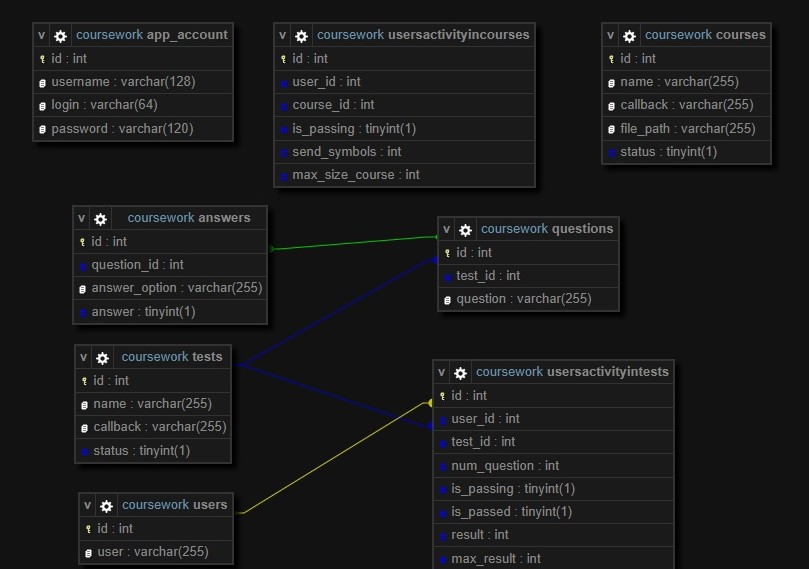
\includegraphics[width=0.8\linewidth]{БД.jpg}}
\caption{База данных и её связи}
\label{fig:БД.jpg}
\end{figure}
\begin{flushright}
    Приложение Б
\end{flushright}
\addcontentsline{toc}{section}{Приложение Б}
Ссылка на github с проектом: https://github.com/crowartie/coursework.
    \end{document}